% "Станет проще"

\documentclass[a4paper,12pt]{article} % тип документа

% report, book

%  Русский язык

\usepackage[T2A]{fontenc}			% кодировка
\usepackage[utf8]{inputenc}			% кодировка исходного текста
\usepackage{graphicx}
\usepackage[english,russian]{babel}	% локализация и переносы


%отступ
\usepackage[left=1cm,right=1cm,
    top=2cm,bottom=2cm,bindingoffset=0cm]{geometry}

% Математика
\usepackage{amsmath,amsfonts,amssymb,amsthm,mathtools} 
\usepackage{csvsimple}
\usepackage{multirow}

\usepackage{hyperref}
\usepackage{wasysym}
\usepackage{subcaption}
\usepackage{verbatim}
\usepackage{hyperref}
\usepackage{float}
\usepackage{enumerate}
\usepackage[dvipsnames]{xcolor}
\usepackage{rotating}
\usepackage{textcomp}

%Заговолок
%\graphicspath{ {images/} }


\begin{titlepage}
\author{Соловьянов Михаил }
\title{Задание 33. Задачи на Влажность.}
\date{\today}
\end{titlepage}



\begin{document} % начало документа
\maketitle
%http://easyfizika.ru/zadachi/elektrostatika/

\section{Задачи попроще}
\subsection{}
Закрытый сосуд объёмом $ V_1 = 0,5 m^3 $ содержит воду массой m = 0,5 кг. Сосуд нагрели до температуры t = 147 °С. На сколько следует изменить объём сосуда, чтобы в нём содержался только насыщенный пар? Давление насыщенного пара рн. п при температуре t = 147 °С равно $4,7 • 10^5$ Па.

%Активная ссылка на источник «Класс!ная физика» обязательна: http://class-fizika.ru/10_a200d.html
\textit{Ответ: $0.3 m^3$}

\subsection{}
 Относительная влажность воздуха в закрытом сосуде при температуре $t_1 = 5$°С равна $\phi_1 = 0.84$, а при температуре $t_2$ = 22 °С равна $\phi_2 = 0.3 $. Во сколько раз давление насыщенного пара воды при температуре $t_2$ больше, чем при температуре $t_1$?

%Активная ссылка на источник «Класс!ная физика» обязательна: http://class-fizika.ru/10_a200d.html
%Активная ссылка на источник «Класс!ная физика» обязательна: http://class-fizika.ru/10_a200d.html

\textit{Ответ: $3$}


\subsection{}

В комнате объёмом $40 m^3$ температура воздуха 20 °С, его относительная влажность $\phi_1 = 0.20$. Сколько надо испарить воды, чтобы относительная влажность $\phi_2$ достигла 0.5 ? Известно, что при 20 °С давление насыщающих паров $Pnp = 2330 $Па.

%Активная ссылка на источник «Класс!ная физика» обязательна: http://class-fizika.ru/10_a200d.html
\textit{Ответ: $0.208$ кг}

\newpage
\section{ Задачи из олимпиады мфтию }

\textit{Цифры возле задач игнорировать.}

\subsection{}

\begin{figure}[h]
\centering
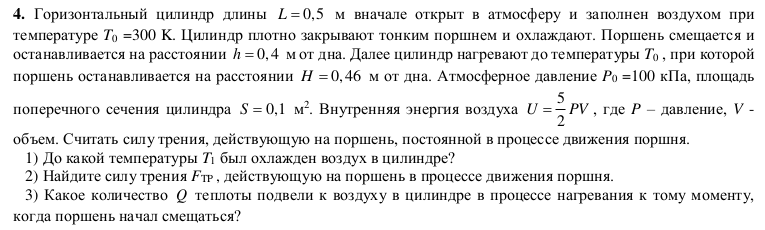
\includegraphics[width=\textwidth]{1.png}
\end{figure}



\subsection{}



\begin{figure}[h]
\centering
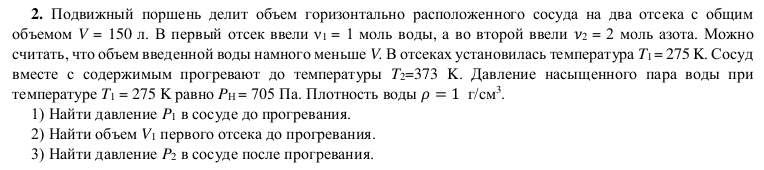
\includegraphics[width=\textwidth]{2.png}
\end{figure}


\end{document}